\section{Context}
    
\frame{\sectionpage}

\begin{frame}{Hired.com: The Market}
    \begin{itemize}
        \item<+-> high-stake recruitment
        \begin{itemize}
            \item[-] most candidates are looking for \textit{\underline{full-time jobs}}: \textcolor{frenchlilac!45!white}{\textbf{96.9\%}} 
            \item[-] \textit{\underline{highly educated}} candidates: \textcolor{frenchlilac!45!white}{\textbf{97.6\%}} bachelor {\tiny and above}, \textcolor{frenchlilac!45!white}{\textbf{41.4\%}} master {\tiny and above}
            \item[-] \textit{\underline{highly paid}} jobs: average annual salary \textcolor{frenchlilac!45!white}{\textbf{\$119,548}}
        \end{itemize} 
        \item<+-> mostly tech industry
        \begin{itemize}
            \item[-] economic significance of tech labor market
            \item[-] substantial gender imbalance: \textcolor{frenchlilac!45!white}{\textbf{20.8\% female}} on Hired.com
        \end{itemize}
    \end{itemize}
\end{frame}

\begin{frame}{Hiring Process on Hired.com}
    \begin{columns}[T]
        \begin{column}{0.3\textwidth}
            \begin{block}{\small \centering \textbf{Ask} Salary}
                \begin{figure}
                    \centering
                    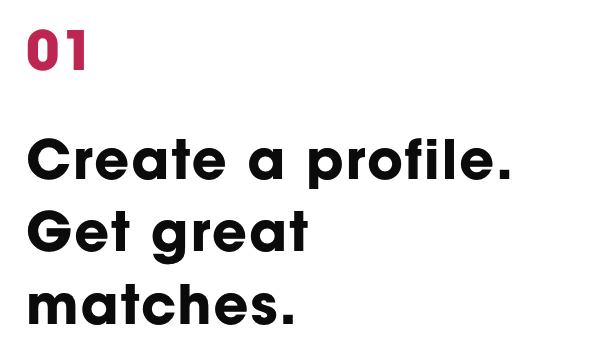
\includegraphics[width = 0.95 \textwidth]{images/hireprocess1.png}
                \end{figure}
            \end{block}
        \end{column}

        \begin{column}{0.3\textwidth}
            \begin{block}{\small \centering \textbf{Bid} Salary}
                \begin{figure}
                    \centering
                    
\includegraphics[width = 0.95 \textwidth]{images/hireprocess2.png}
                \end{figure}
            \end{block}
        \end{column}

        \begin{column}{0.3\textwidth}
            \begin{block}{\small \centering \textbf{Final} Salary}
                \begin{figure}
                    \centering
                    
\includegraphics[width = 0.95 \textwidth]{images/hireprocess3.png}
                \end{figure}
            \end{block}
        \end{column}
    \end{columns}
\end{frame}

\begin{frame}{Supply Side: Jobseekers' Profile}
    \begin{figure}
        \centering
        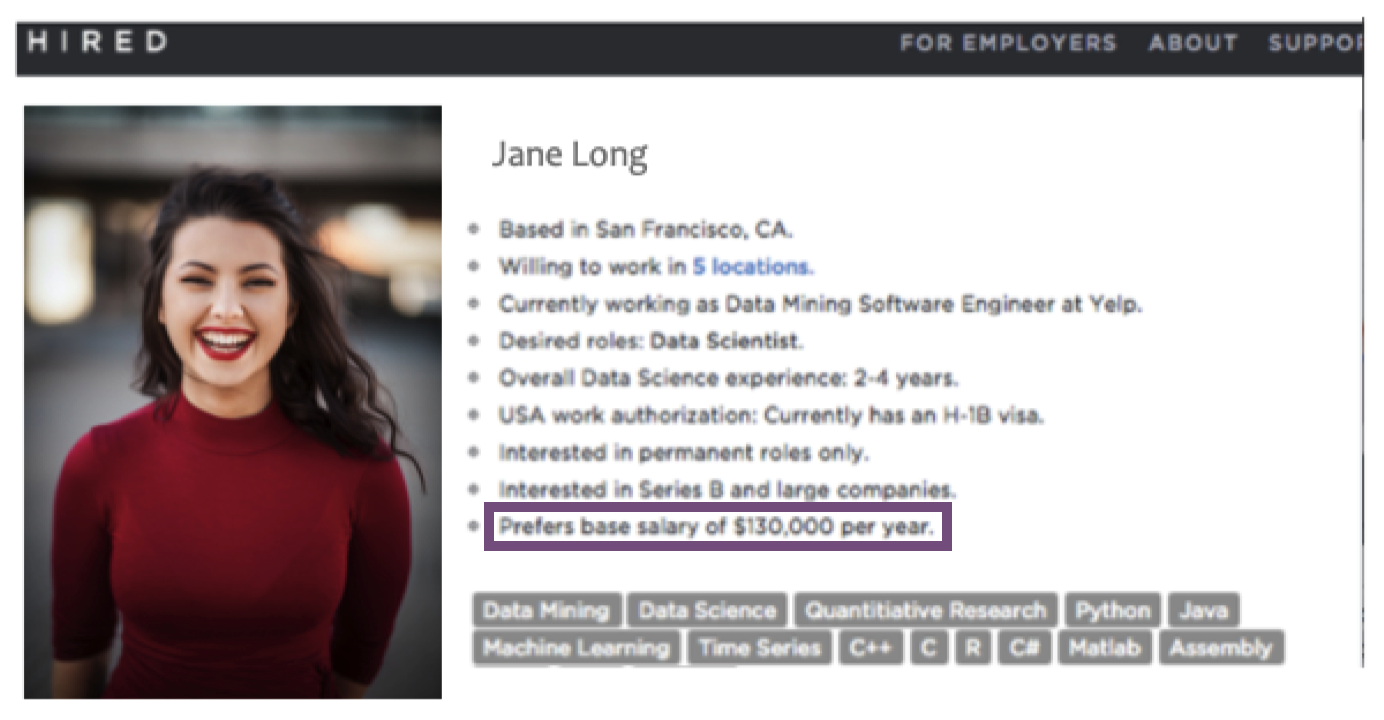
\includegraphics[height = 0.75 \textheight]{images/jobseeker.png}
    \end{figure}
\end{frame}

\begin{frame}{Demand Side: Employers' Interview Request}
    \begin{figure}
        \centering
        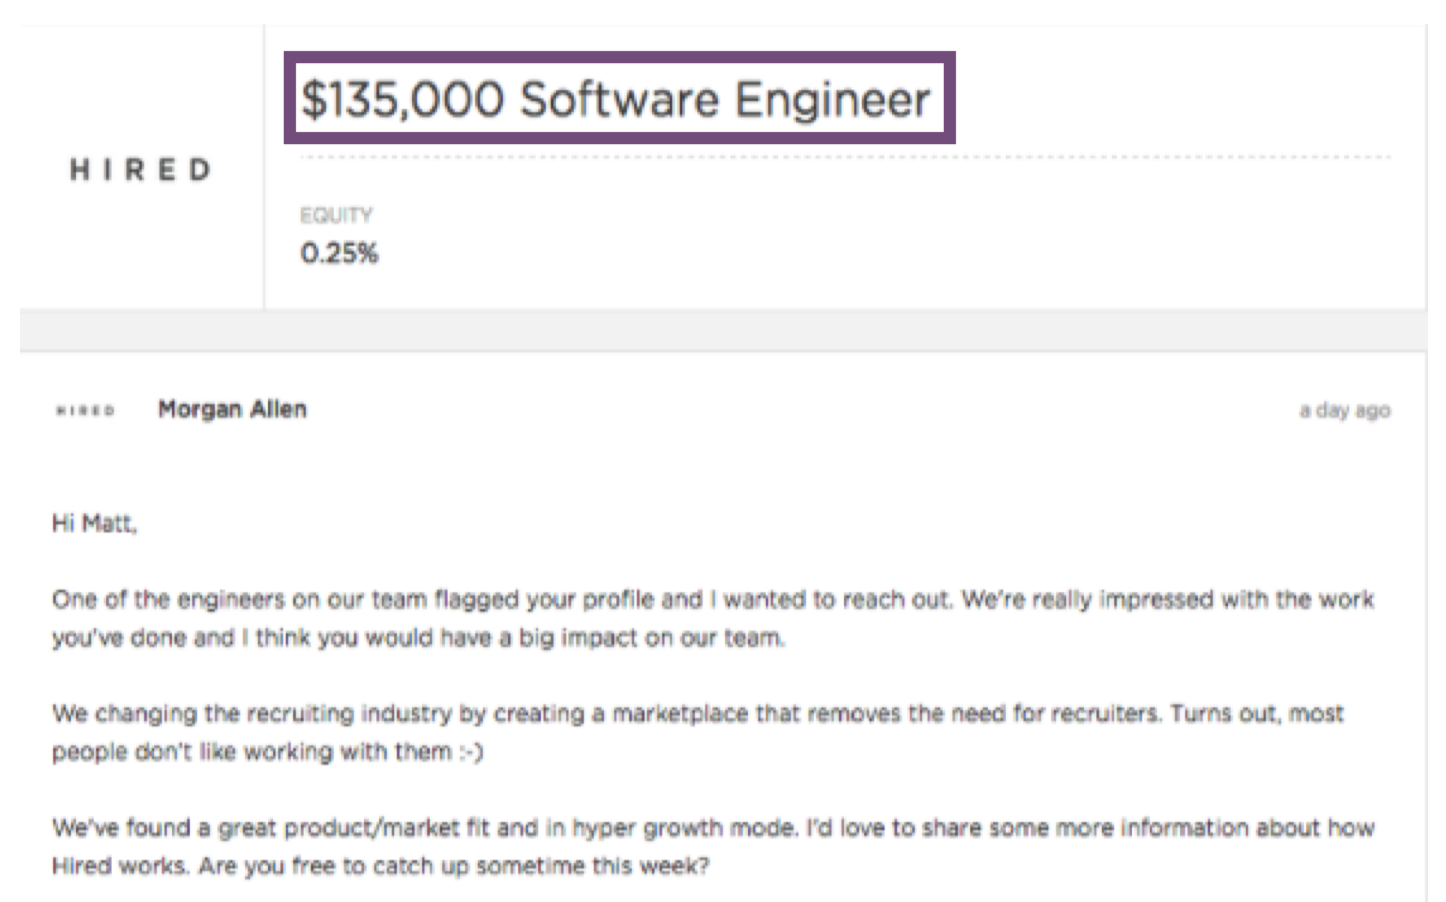
\includegraphics[height = 0.75 \textheight]{images/employer.png}
    \end{figure}
\end{frame}

\begin{frame}{Recap: Hiring Process on Hired.com}
    \begin{figure}
        \centering
        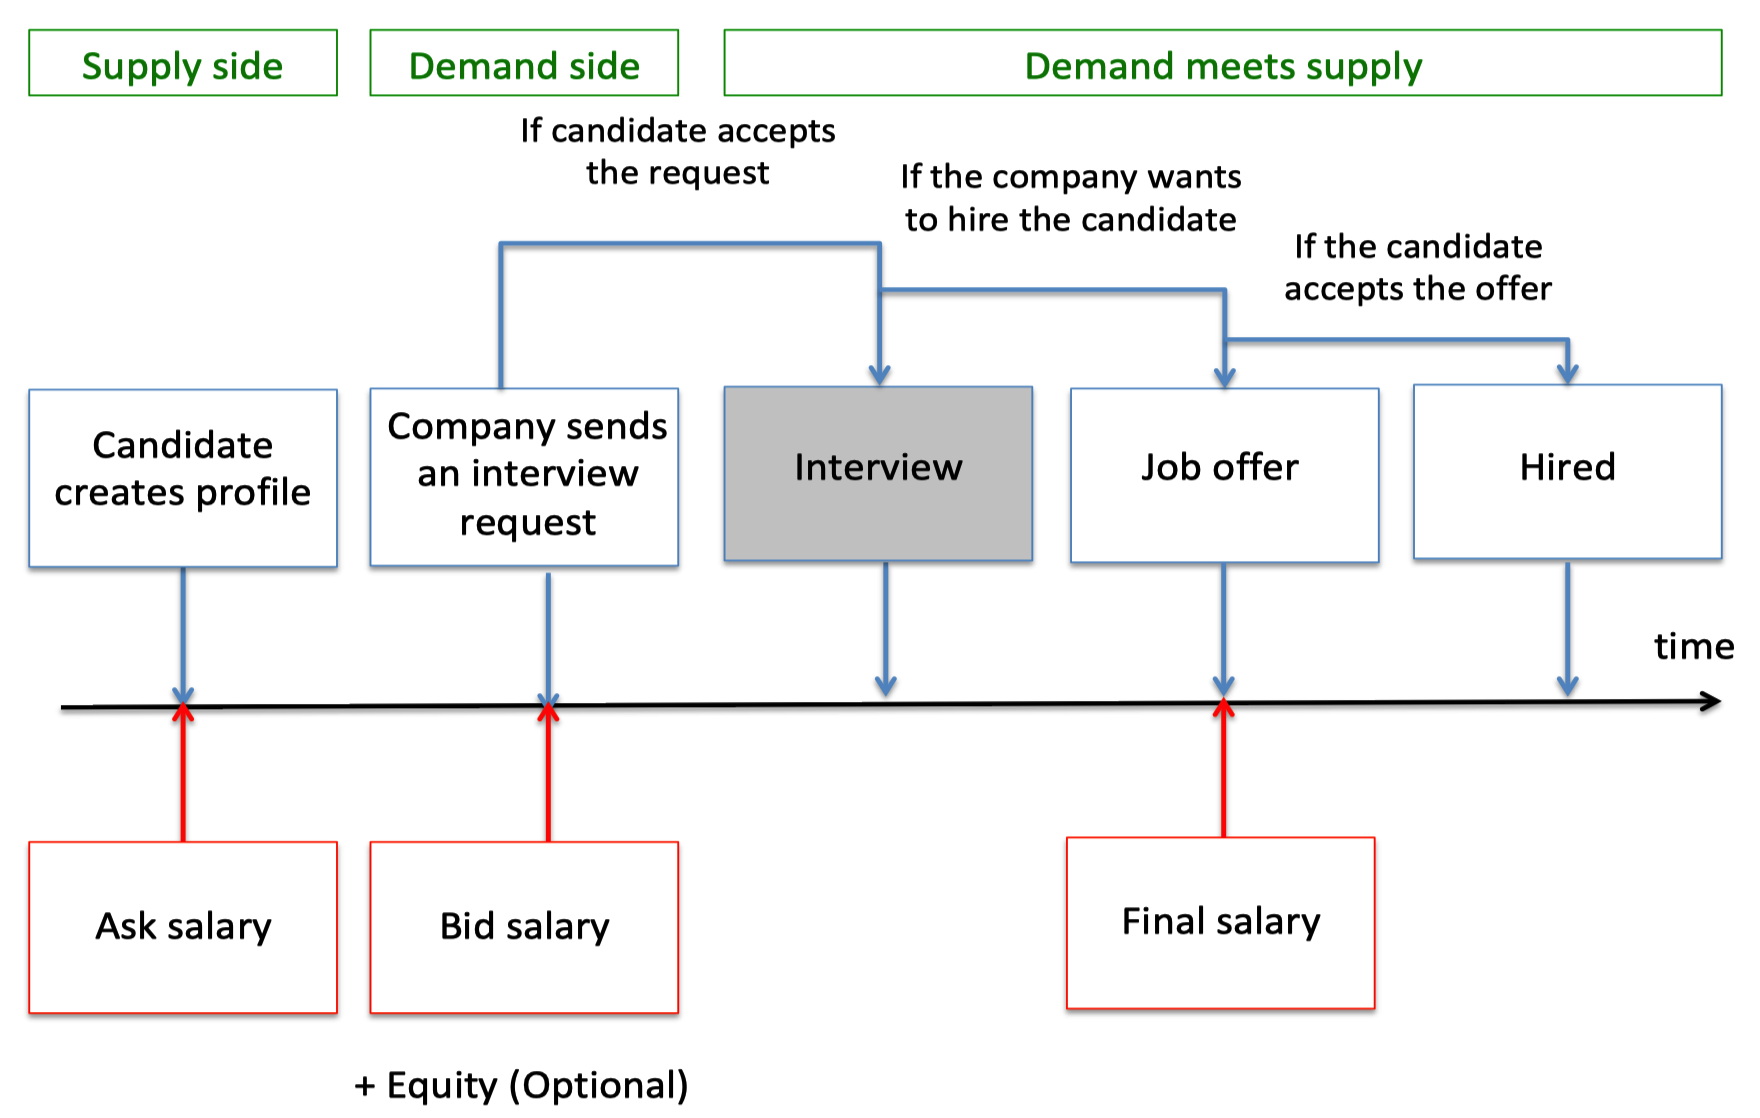
\includegraphics[height = 0.7 \textheight]{images/hiringflow.png}
    \end{figure}
\end{frame}
